\documentclass[a4paper,10pt,twoside,openany]{ltjreport}
\usepackage{fancyhdr}
\usepackage{graphicx}
\usepackage[bookmarks=true,%
  bookmarksnumbered=true,%
  colorlinks=true,%
  linkcolor=blue,%
  citecolor=blue,
  setpagesize=false,unicode]{hyperref}
\usepackage{ascmac}
\usepackage{fancybox}
\usepackage{amsmath,amssymb}
\usepackage{amsfonts}
\usepackage{bm}
\usepackage{algorithm}
\usepackage{algpseudocode}
\usepackage{url}
%\usepackage[top=40truemm,bottom=35truemm,left=40truemm,right=30truemm]{geometry}

\graphicspath{{./graphics/}}
\newcommand{\Alref}[1]{Algorithm~\ref{#1}}
\newcommand{\Equref}[1]{式~(\ref{#1})}
\newcommand{\Figref}[1]{図~\ref{#1}}
\newcommand{\mb}{\mathbf}
\newcommand{\mr}{\mathrm}
\DeclareMathOperator*{\argmin}{arg\,min}
\DeclareMathOperator*{\argmax}{arg\,max}

\bibliographystyle{junsrt}
\renewcommand{\bibname}{参考文献}

\def\name{\color{red}{学籍番号 名前}}
\def\ttl{\color{red}{タイトル}}

\title{2015年度修士論文\\\ttl}
\author{早稲田大学 先進理工学研究科\\電気・情報生命専攻\\情報学習システム研究室\\\leavevmode\\\name}
\date{\today}

% -------------- PAGE STYLE SETTINGS ---------------
\pagestyle{fancy}
\fancyhead{}
\fancyhead[RO,RE]{\rightmark}
\fancyhead[LE,LO]{\leftmark}
\fancyfoot{}
\fancyfoot[LE,RO]{\thepage}
\renewcommand{\chaptermark}[1]{\markboth{第\ \thechapter\ 章~#1}{}}
\renewcommand{\sectionmark}[1]{\markright{\thesection~#1}{}}

\setlength{\hoffset}{-0.0in}
\setlength{\voffset}{5.0mm}
\setlength{\textheight}{580pt}
\setlength{\oddsidemargin}{12.4mm}% 20mm - 1in
\setlength{\evensidemargin}{10.4mm}% 20mm - 1in
\setlength{\textwidth}{135mm}
\setlength{\headwidth}{145mm}
\renewcommand{\headrulewidth}{0.4pt}
\renewcommand{\footrulewidth}{0.4pt}
% ------------ PAGE STYLE SETTINGS END --------------

\begin{document}

\maketitle

\tableofcontents
% \listoftables
% \listoffigures

\chapter{序章}
\section{背景}
睡眠は脳によって制御されており\cite{Hobson2005},哺乳類にとって必要不可欠な生理現象である.
その重要性にも関わらず,睡眠について解明されていないことが多い.
その中でも,睡眠とはいかなる生物学的な状態か,という問いに対する明確な答えは未だない\cite{Kanda2016}.

哺乳類の睡眠状態は脳波によって定義される.
しかし,哺乳類以外は脳波を計測することができないためふるまいでしか評価できない.
そこで,ニューロンの活動から睡眠を新たに定義することができれば睡眠状態の解明に繋がると考えられる\cite{Kanda2020}.

脳内の情報伝達は複数個のニューロンによって行われている.
また,睡眠時には多数のニューロンが活動してある現象が見られることが知られている.
複数ニューロンの活動を解析することが重要である.

ニューロンの観察方法として,パッチクランプ法,細胞内記録法,細胞外記録法などの電気生理学的な手法が挙げられる.
これらの手法は十分な時間分解能かつ細胞レベルでニューロンを観察することができる.
しかし,電気生理学的な手法では観察できるニューロンの数は数十から多くても数百程度である.

より多くのニューロンを観察するために,蛍光イメージングの1つであるカルシウムイメージングという手法が用いられる.
ニューロンで活動電位が発生(発火)すると細胞内の$\text Ca^{2+}$濃度が上昇する.
カルシウムイメージングでは,この$\text Ca^{2+}$濃度上昇を蛍光で可視化する.
具体的には,$\text Ca^{2+}$と結合すると蛍光強度が変化する蛍光分子を細胞内に発現させておき,$\text Ca^{2+}$濃度を蛍光強度として蛍光顕微鏡で観察する.
蛍光イメージングを用いる利点として,(1)高い空間分解能,(2)広い観察範囲,(3)遺伝子工学と併用して興奮性/抑制性ニューロンの同定などをした上での観察ができることが挙げられる.
一方,時間分解能が電気生理学的手法よりも低いことが蛍光イメージングの欠点である.
$\text Ca^{2+}$濃度の変化はニューロンの電気的変化よりも遅く,また,カルシウム感受性蛍光分子のキネティクスも影響する.
さらに,カメラやレーザースキャンでのサンプリングレートは高くても100Hz程度であり,ニューロンの個々の発火を全て捉えるには不十分である.

本研究で扱うデータは,8Hzのサンプリングレートで観察された100〜200個のマウスのニューロンのカルシウムイメージングデータである.
本研究では,低い時間分解能のカルシウムイメージングデータからニューロンをクラスタリングし,人工データ実験を通してどの程度の情報が抽出できるかを確認する.

% \include{theory}
% \include{formulization}
% \include{estimate}
% \include{experiment}
% \include{conclusion}

\bibliography{../../../BibTeX/library.bib}

% \chapter{付録 人工データ}
\section{シミュレーション}
ニューロン集団のカルシウムイメージングデータをシミュレーションによって作り,解析手法を評価する.
シミュレーションでは1)ニューロンのネットワーク構造を作成し,2)スパイクのシミュレーションを行い,3)蛍光強度の観測データに変換する.
\subsection{ネットワーク構造}
シミュレーションに用いるニューロンの個数を$N$として,ニューロンのネットワーク構造を$S \in {0, 1}^{N \times N}$とする.
$s_{ij}$はニューロン$i$からニューロン$j$へ活動電位が伝わるかを表している.
本節では$S$の作り方を説明する.

ニューロンのネットワーク構造にはsmall world network\cite{Watts1998}を用いる.
Small world networkはノード数,張り替え確率,初期次数を決めることによってネットワークを作成するアルゴリズムである.
初期次数は,ニューロンが平均何個のニューロンとシナプス結合を持つかという変数である.
張り替え確率は,初期次数によって作成された規則的なグラフのエッジをランダムに張り替える確率である.
そのため,エッジのうち何割が遠くのニューロンとつながっているかを表す変数である.

実際のニューロンをsmall world networkによって表すために,初期次数と張り替え確率を実データから決める.
今回はこの値はニューロンのコネクションの割合と相互のコネクションの割合から決める.
興奮性ニューロン同士の6.7\%であり,そのうち双方向のコネクションの割合は24\%である\cite{Jouhanneau2015}.
発達中マウスの興奮性ニューロンから抑制性ニューロンへのコネクティビティと抑制性ニューロンから興奮性ニューロンへのコネクティビティはどちらも78\%であった\cite{Holmgren2003}.
成熟したマウスではより少ないと思われるが,データが見つからなかったため,40\%とした.
相互のコネクションの割合がランダムにエッジを作るよりも高いのは,近いニューロンにコネクションが作られやすいからだと考えられる.
これらのデータを実現するように初期次数と張り替え確率を調整した.
用いたパラメータを\Tabref{tab:parameter1}に示す.
抑制性ニューロン同士のコネクティビティは分からないため,興奮性ニューロンと同じにしている.

\begin{table}[htb]
  \center
  \begin{tabular}{|c|cc|} \hline
    結合の種類 & 初期次数 & 張り替え確率 \\ \hline
		同種類のニューロン間 & $0.0335 N$ & $0.3$ \\
		興奮性ニューロンと抑制性ニューロン間 & $0.2N$ & $0.3$\\ \hline
  \end{tabular}
  \caption{ネットワーク構造のパラメータ}
  \label{tab:parameter1}
\end{table}

実際のネットワーク構造の作り方を説明する.
ネットワーク構造は興奮性ニューロン同士の結合,抑制性ニューロン同士の結合,興奮性ニューロンと抑制性ニューロン間の結合の3つに分けて作成する.
まず,全ニューロンのうち抑制性ニューロンと興奮性ニューロンのインデックスを決めておく.
全てのニューロンについて\Tabref{tab:parameter1}に従ってネットワークを作成し,それぞれに対応する隣接行列の上三角または下三角行列を取り出して結合する.
作成したいのは向きのある有向グラフなので,上三角行列と下三角行列を分けて作成する.

\subsection{スパイクシミュレーション}
スパイクのシミュレーションにIzhikevichモデル~\cite{Izhikevich2003}を用いる.
このモデルはHodgikin-Huxleyモデルをもとにしており,計算コストが低い.
Izhikevichモデルでは,あるニューロンの膜電位が閾値を超えると発火したとみなし,あらかじめ定義したニューロンのネットワーク構造に従って結合を持つニューロンの膜電位を上昇させる.
このシミュレーションで設定しなければいけないのは,個々のニューロンの特徴パラメータ,重み付きのネットワーク構造,外部からのランダムな入力である.

まず,個々のニューロンの特徴パラメータについて説明する.
このモデルではニューロンごとに4つのパラメータを設定する必要があり,そのパラメータでニューロンを特徴づける.
本論文では興奮性ニューロンにはregular spiking neurons,抑制性ニューロンにはfast spiking neuronsを用いる.
それらのパラメータを~\Tabref{tab:parameter2}に示す.
ただし,$r_e$と$r_i$は0から1の一様分布に従う確率変数である.

\begin{table}[htb]
  \center
  \begin{tabular}{|c|cccc|} \hline
    ニューロンの種類 & a & b & c & d \\ \hline
    興奮性ニューロン & 0.02 & 0.2 & $-65 + 15 r_e^2$ & $8 - 6r_e^2$ \\
    抑制性ニューロン & $0.02 + 0.08r_i$ & $0.25 - 0.05 r_i$ & -65 & 2 \\ \hline
  \end{tabular}
  \caption{Izhikevichモデルのパラメータ}
  \label{tab:parameter2}
\end{table}

次に,重み付きのネットワーク構造$W \in \mathbb{R}^{I \times I}$について説明する.
ニューロン$i$から$j$へ結合があった場合,$w_{ij}$はニューロン$i$が発火した時にニューロン$j$の膜電位をどれだけ上昇させるかという数値である.
$W$は,前節で作成した$S$の非ゼロ要素を数値で置き換えることで作成する.
興奮性ニューロンからの結合は一様分布$U(0, 0.5)$からサンプルし,抑制性ニューロンからの結合は一様分布$U(-2,0)$からサンプルする.
\begin{align}
	w_{ij} = \begin{cases}
		U(0,0.5) & (s_{ij} = 1 \ and \ i \in \ excitatory \ neuron) \\
		U(-2,0) & (s_{ij} = 1 \ and \ i \in \ inhibitory\  neuron) \\
		0 & (s_{ij} = 0)
  \end{cases}
	\label{eq:W}
\end{align}

最後に外部からのランダムな入力について説明する.
ニューロンには観測範囲外からの入力がある(以降,外部入力とする).
そのため,シミュレーション中も外部からの電位を乱数としてニューロンの電位に足す.
本論文では,ニューロンの活動も外部入力の大きさで表現する.
活動していない興奮性ニューロンと抑制性ニューロンにはそれぞれ,$\mathcal{N}(0,5)$と$\mathcal{N}(0,2)$に従う乱数を足す.
活動している興奮性ニューロンと抑制性ニューロンにはそれぞれ,$\mathcal{N}(1,5)$と$\mathcal{N}(0.4,2)$に従う乱数を足す.
これらを\Tabref{tab:parameter3}に示す.
活動していないニューロンへの外部入力は\cite{Izhikevich2003}で用いられていたものを採用した.
ただし,興奮性ニューロンの活動時の外部入力は変化させた実験もある.

\begin{table}[htb]
  \center
  \begin{tabular}{|c|cc|} \hline
    ニューロンの種類 & 活動時の外部入力 & 活動していない時の外部入力 \\ \hline
		興奮性ニューロン & $\mathcal{N}(0.8,3)$ & $\mathcal{N}(0, 5)$ \\
		抑制性ニューロン & $\mathcal{N}(0.4, 0.1)$ & $\mathcal{N}(0, 2)$ \\ \hline
  \end{tabular}
  \caption{シミュレーションに用いる外部入力の値}
  \label{tab:parameter3}
\end{table}

本論文では同時に活動するニューロンを推定するのが目的の1つである.
ある時間帯にあるニューロングループが活動する時,そのニューロングループには平均値を上げた外部入力を足し,それ以外のニューロンには平均$0$の外部入力を足す.
こうすることで,ニューロングループの活動のみ上がる(つまり蛍光強度が上がる).
実際の脳でもこのように外部からの入力によってニューロンの活動を制御していると考えられる.
あるニューロングループを活動させるには,そのグループのハブとなるニューロンにのみ強い外部入力を与える方法も考えられるが今回は採用しない.
なぜなら,ネットワーク構造をかなり工夫しないと実現できないためである.

実際にマウスのニューロンの発火頻度がどれくらいなのか\cite{Watson2016}を元に\Tabref{tab:spike-frequency}に示す.
\begin{table}[htb]
  \center
  \begin{tabular}{|c|ccc|} \hline
    ニューロンの種類 & 覚醒時(Hz) & ノンレム睡眠時(Hz) & レム睡眠時(Hz) \\ \hline
		興奮性ニューロン & $0.76 \pm 1.53$ & $0.69 \pm 0.86$ & $0.88 \pm 1.33$ \\
		抑制性ニューロン & $5.59 \pm 7.25$ & $4.69 \pm 5.62$ & $4.25 \pm 9.43$ \\ \hline
  \end{tabular}
  \caption{ニューロンごとの発火頻度の中央値}
  \label{tab:spike-frequency}
\end{table}

\subsection{カルシウムイメージングモデル}
スパイクデータからカルシウムイオン濃度を計算する~\cite{Vogelstein2009}のモデルを用いる:
\begin{equation}
  [Ca^{2+}]_{i,t} - [Ca^{2+}]_{i,t-1} = - \frac{\Delta}{\tau}([Ca^{2+}]_{i,t-1} - [Ca^{2+}]_b) + An_{i,t} + \sigma_c \sqrt{\Delta} \epsilon_{i,t},
  \label{eq:calcium}
\end{equation}
ただし,$[Ca^{2+}]_{i,t}$をニューロン$i$の時刻$t$でのカルシウムイオン濃度,$[Ca^{2+}]_b$をカルシウムイオン濃度のベースライン,$\Delta$を時間幅,$\tau$は時定数,$A$は1つのスパイクでのカルシウムイオン濃度の上がり幅,$n_{i,t} \in \{0,1\}$はニューロン$i$の時刻$t$でのスパイク,$\sigma_c$はノイズの分散,$\epsilon_{i,t}$は標準正規分布に従う確率変数である.
この人工データではsaturationは考えないこととする.

次に,同論文のモデルを使ってカルシウムイオン濃度$[Ca^{2+}]_{i,t}$をカルシウムイメージングで計測される蛍光強度$F_{i,t}$に変換する:
\begin{equation}
	F_{i,t} = \alpha[Ca^{2+}]_{i,t} + \beta + \sigma_F \epsilon_{i,t},
  \label{eq:intensity}
\end{equation}
$\alpha$は強度,$\beta$はバイアス,$\sigma_F$はノイズの分散である.
\Tabref{tab:parameter2}に使用したパラメータを示す.
何種類かの蛍光タンパク質の性能を調べた論文に\cite{Chen2013a}がある.
この論文の,1秒間に10回発火した時のdecay time(蛍光強度が上がり切ってから半分の強度になるまでの時刻)から$\tau = 2.3$とし,SN比から$\sigma_c = 0.5$とした.

\begin{table}[htb]
  \center
  \begin{tabular}{|cccccccc|} \hline
    $[Ca^{2+}]_b$ & $\Delta$ & $\tau$ & $A$ & $\sigma_c$ & $\alpha$ & $\beta$ & $\sigma_F$ \\ \hline
    0.1 & 0.001 & 2.3 & 5.0 & 0.5 & 1.0 & 10 & 1.0 \\ \hline
  \end{tabular}
  \caption{カルシウムイメージングモデルでのパラメータ}
  \label{tab:parameter2}
\end{table}

\subsection{観測モデル}
実データは8[Hz]でサンプリングされたデータなので,シミュレーションした蛍光強度を8[Hz]で足し合わせる:
\begin{equation}
  x_{i,t'} = \sum_{t=1}^{125} F_{i,t},
  \label{eq:observation}
\end{equation}
ここで,$t'$はサンプリング後の時刻を表す.

上記の方法で作成した人工データ時系列と観測時系列をそれぞれ\Figref{fig:art}と\Figref{fig:dat}に示す.
\begin{figure}[htbp]
    \begin{minipage}{0.5\hsize}
			\begin{center}
					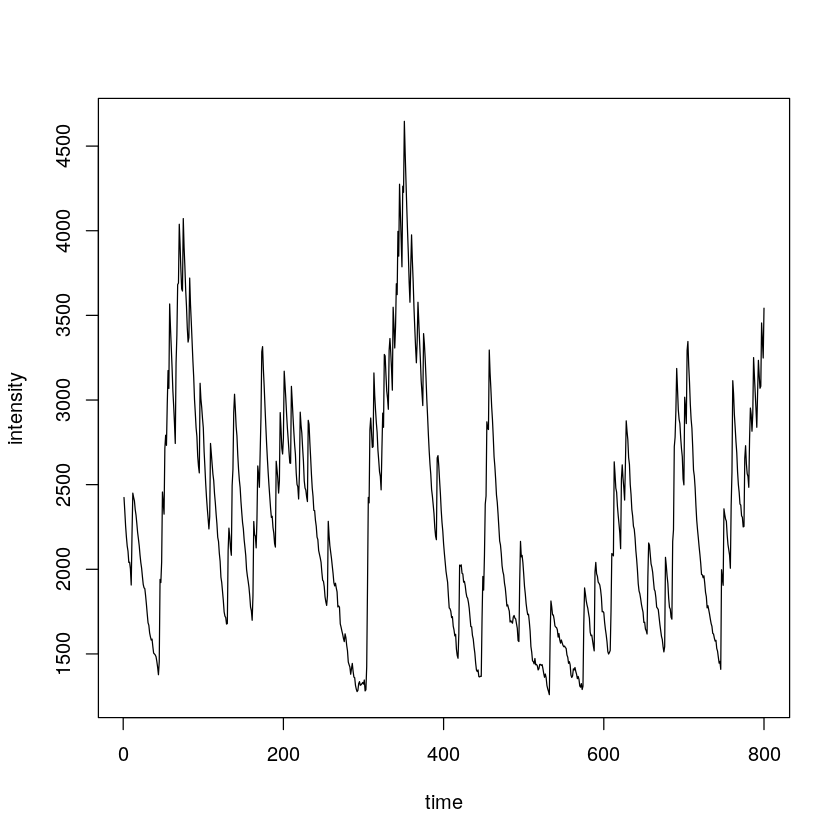
\includegraphics[width=\hsize]{artificial_data}
					\caption{1つのニューロンの人工時系列.}
					\label{fig:art}
			\end{center}
		\end{minipage}
    \begin{minipage}{0.5\hsize}
			\begin{center}
					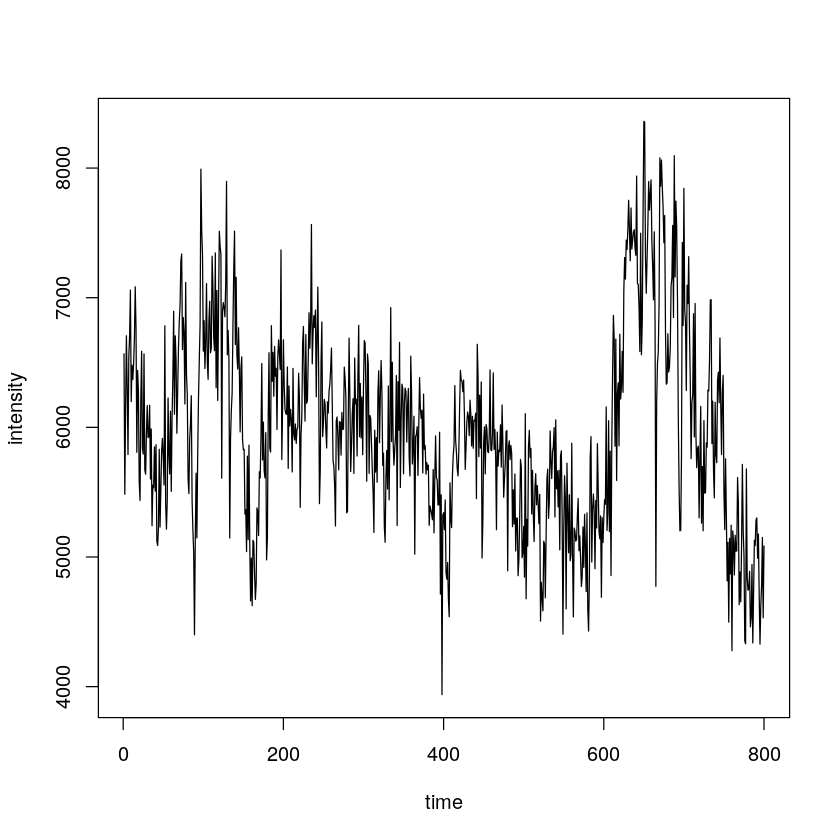
\includegraphics[width=\hsize]{real_data}
					\caption{1つのニューロンの観測時系列.}
					\label{fig:dat}
			\end{center}
		\end{minipage}
\end{figure}


\end{document}
